\cleardoublepage

\chapter{Visualización Científica}
\label{makereference4}

En este capítulo se muestran técnicas relevantes de visualización científica.
Algunas de ellas serán implementadas mediante shaders en nuestra aplicación,
explicando los shaders utilizados en ella.

\section{Manipulación de imágenes}
\label{ref:images}

% Incluir imágenes de las diferentes manipulaciones
% TODO

La manipulación de imágenes es la disciplina que incluye las diferentes técnicas
de filtrado, combinación o modificación de imágenes con el fin de resaltar
características deseables de la imagen. En visualización científica, por
ejemplo, se puede utilizar el negativo de la imagen de una estructura ósea con
el fin de detectar defectos que de otro modo resulta más complicado ver;
utilizar una mezcla de imágenes astronómicas en diferentes espectros para
conseguir una imagen mas realista; o aumentar el brillo y nitidez de una imagen
para conseguir una visualización más eficaz. 

Entre estas técnicas podemos encontrar, por ejemplo:

\begin{itemize}
		\item Negativo
		\item Detección de bordes
		\item Cambios de brillo, contraste y nitidez
		\item Mezcla de imágenes
\end{itemize}

\section{Curvas y superficies de Bézier}
\label{ref:bezier}

Se denominan curvas de Bézier a un sistema de trazado de dibujos técnicos ideado
en los años 60 por Pierre Bézier. El modelo se basa en una descripción
matemática que se utiliza extensivamente en programas tipo CAD, y son muy útiles
para modelar curvas suaves y fáciles de manipular mediante sus puntos de
control. Éstas pueden ser, generalmente, lineales, cuadráticas o cúbicas, aunque
se puede generalizar a cualquier grado. 

Las curvas de Bézier vienen definidas mediante el llamado Polinomio de Bézier
$B(t)$ y el grado de este polinomio es el que determina el grado de la curva.
Las curvas de Bézier lineales tienen dos puntos de control $\mathbf{P_0}$ y
$\mathbf{P_1}$, por lo que la curva resultante es en realidad una recta entre
esos dos puntos. Siguen la fórmula general de una recta, es decir:

\begin{equation}
	B(t) = \mathbf{P_0} + (\mathbf{P_1} - \mathbf{P_0})t = (1 - t)\mathbf{P_0} +
	t\mathbf{P_1}, \; t \in [0,1] \label{eq:1}
\end{equation}

Las cuadráticas tienen tres puntos de control $\mathbf{P_0}$, $\mathbf{P_1}$ y $\mathbf{P_2}$ y sigue la
trayectoria marcada por la función $B(t)$:

\begin{equation}
	B(t) = (1 - t)^2\mathbf{P_0} + 2t(1-t)\mathbf{P_1} + t^2\mathbf{P_2}, \; t
	\in [0,1] \label{eq:2}
\end{equation}

En las curvas cúbicas se utilizan cuatro  puntos de control $\mathbf{P_0}$,
$\mathbf{P_1}$, $\mathbf{P_2}$ y $\mathbf{P_3}$, siguiendo la trayectoria:

\begin{equation}
	B(t) = (1 - t)^3\mathbf{P_0} + 3t(1-t)^2\mathbf{P_1} + 3t^2(1-t)\mathbf{P_2}
	+ t^3\mathbf{P_3}, \; t \in [0,1] \label{eq:3}\\
\end{equation}

Si generalizamos este polinomio se pueden generar curvas de grado $n$ siguiendo
la fórmula:

\begin{equation}
	B(t) = \sum_{k = 0}^{n}\mathbf{P_k}BEZ_{k,n}(t) , \; t \in [0,1] \label{eq:4}
\end{equation}

donde $BEZ_{k,n}(t)$ son conocidos como los polinomios de Bernstein:

\begin{equation}
	BEZ(t) = \binom{n}{k}t^k(1-t)^{n-k}, \; k=0,\ldots,n \label{eq:5}
\end{equation}

En cuanto a las superficies de Bézier, se generan mediante dos conjuntos de
curvas de Bézier ortogonales, especificadas mediante una malla de puntos de
control. La ecuación para estas superficies es:

\begin{equation}
B(t, u) =
\sum_{j=0}^{m}{\sum_{k=0}^{n}{\mathbf{P_{j,k}}BEZ_{j,m}(t)BEZ_{k,n}(u)}}
\label{eq:6}
\end{equation}

Las curvas y superficies de Bézier tienen propiedades muy interesantes, como la
posibilidad de calcular las primeras y segundas derivadas de la curva en los
puntos finales, posibilitando su empalme con otras curvas suavemente. Para leer
más acerca de las curvas y superficies de Bézier se pueden
consultar~\citet{HEARN,Bailey}.

\begin{figure}[t]
		\centering
	\begin{subfigure}[b]{.3\textwidth}
			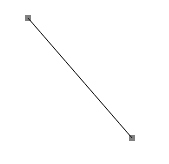
\includegraphics[height=5cm,width=\textwidth]{figures/bezier1.png}
			\caption{Lineal}
			\label{fig:bezier1}
	\end{subfigure}
	\begin{subfigure}[b]{.3\textwidth}
			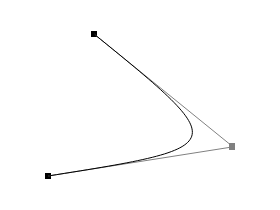
\includegraphics[height=5cm,width=\textwidth]{figures/bezier2.png}
			\caption{Cuadrática}
			\label{fig:bezier2}
	\end{subfigure}
	\begin{subfigure}[b]{.3\textwidth}
			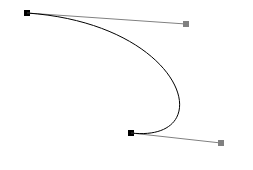
\includegraphics[height=5cm,width=\textwidth]{figures/bezier3.png}
			\caption{Cúbica}
			\label{fig:bezier3}
	\end{subfigure}
	\caption{Curvas de Bézier.}
	\label{fig:bezier}
\end{figure}

\begin{figure}[t]
	\centering	
	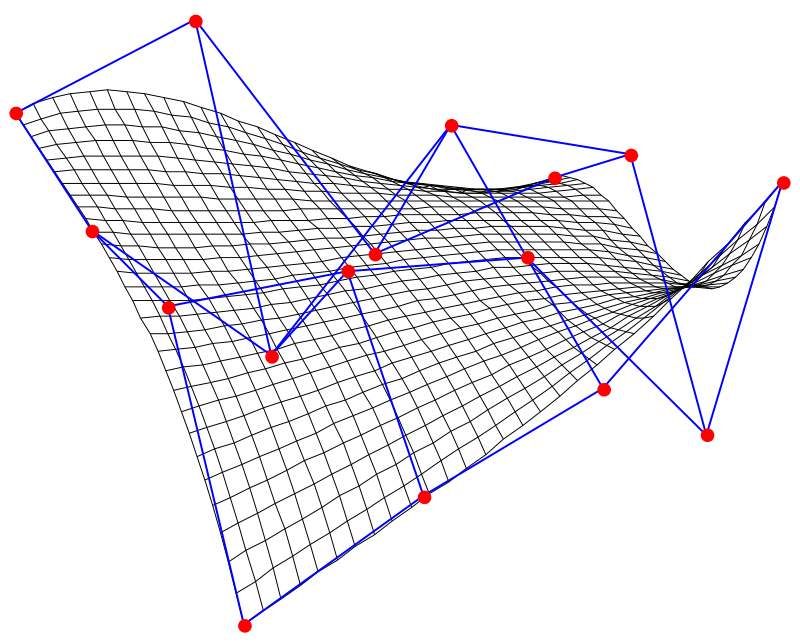
\includegraphics[height=8cm]{figures/beziersurface.png}
	\caption[Superficie de Bézier con 16 puntos de control.]{Superficie de
	Bézier con 16 puntos de control. Fuente:~\cite{bsurfaceimage}}
	\label{fig:beziersurface}
\end{figure}

\section{Visualización de datos en 3D}
\label{ref:cloud}

Otra de las grandes áreas de la visualización científica es la de visualizar
conjuntos grandes de datos en tres dimensiones. Estos datos pueden ser tanto
escalares como vectoriales. Por ejemplo, se pueden monitorizar los datos de
temperatura en la atmósfera durante un determinado período de tiempo, queriendo
después visualizar las áreas que han estado más calientes de media. 

Otro tipo de visualización de datos en tres dimensiones es la visualización de
datos vectoriales en tres dimensiones, con el fin de capturar, por ejemplo,
flujos vectoriales de fluidos al rededor de un objeto, etc.

Para este tipo de tareas existen diferentes métodos de visualización, entre los
que se encuentran los siguientes:

\begin{itemize}
	\item Nubes de puntos (Figura~\ref{fig:pointcloud})
	\item Visualización de volumen (Figura~\ref{fig:volumevisualization})
	\item Isosuperficies (Figura~\ref{fig:isosurface})
	\item Planos cortados (Figura~\ref{fig:sliceplanes})
	\item Trazado de partículas (Figura~\ref{fig:particletracing})
	\item Visualización de vectores en 3D  (Figura~\ref{fig:vectorvisualization})
\end{itemize}

\begin{figure}[t]
	\centering
	\begin{subfigure}[b]{.45\textwidth}
			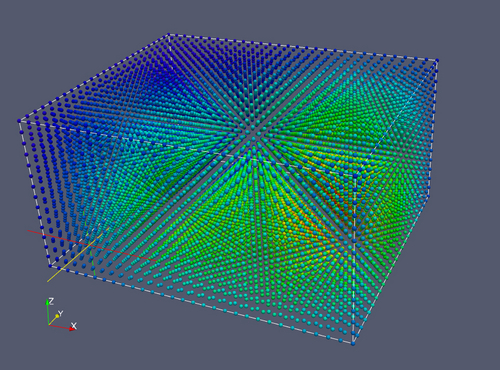
\includegraphics[height=6cm,width=\textwidth]{figures/pointcloud.jpg}
			\caption{Nube de puntos}
			\label{fig:pointcloud}
	\end{subfigure} \hfill
	\begin{subfigure}[b]{.45\textwidth}
			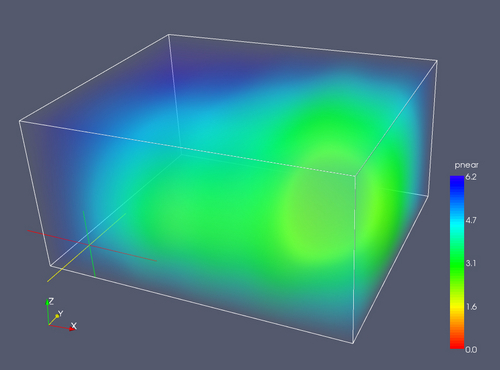
\includegraphics[height=6cm,width=\textwidth]{figures/volumevisualization.jpg}
			\caption{Visualización de volumen}
			\label{fig:volumevisualization}
	\end{subfigure}
	\newline \\
	\begin{subfigure}[b]{.45\textwidth}
			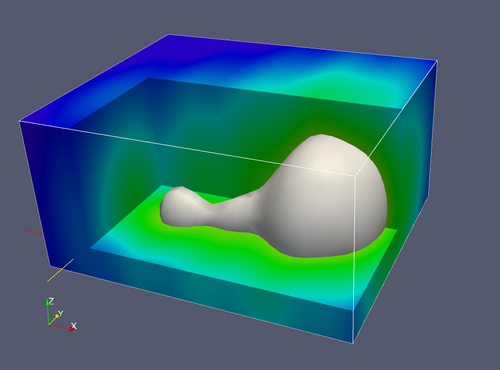
\includegraphics[height=6cm,width=\textwidth]{figures/isosurface.jpg}
			\caption{Isosuperficie}
			\label{fig:isosurface}
	\end{subfigure} \hfill
	\begin{subfigure}[b]{.45\textwidth}
			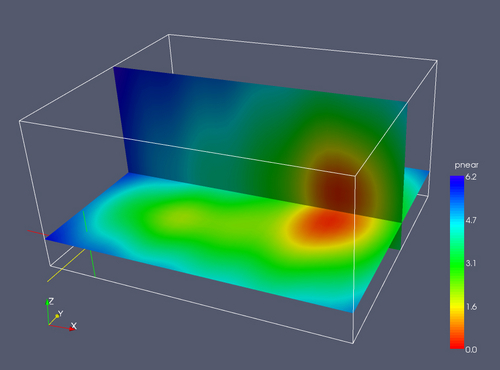
\includegraphics[height=6cm,width=\textwidth]{figures/sliceplanes.jpg}
			\caption{Planos cortados}
			\label{fig:sliceplanes}
	\end{subfigure}
	\newline\\
	\begin{subfigure}[b]{.45\textwidth}
			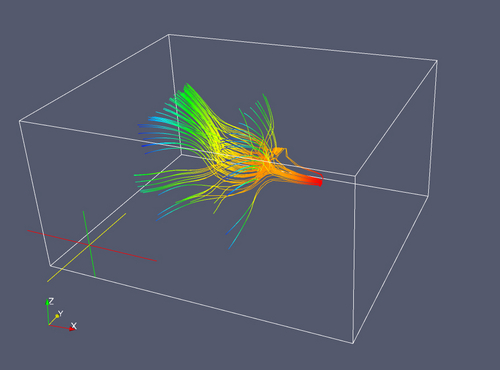
\includegraphics[height=6cm,width=\textwidth]{figures/particletracing.jpg}
			\caption{Trazado de partículas}
			\label{fig:particletracing}
	\end{subfigure} \hfill
	\begin{subfigure}[b]{.45\textwidth}
			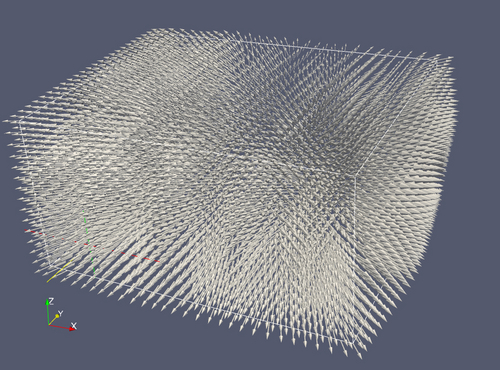
\includegraphics[height=6cm,width=\textwidth]{figures/vectorvisualization.jpg}
			\caption{Visualización de vectores}
			\label{fig:vectorvisualization}
	\end{subfigure}
	\caption[Técnicas de visualización en 3D.]{Técnicas de visualización en 3D. Fuente:~\cite{3dimages}}
	\label{fig:3dvis}
\end{figure}

\section{Sólidos de revolución}
\label{ref:revolution}

Los sólidos de revolución han sido siempre objeto de estudio en matemáticas,
física e ingeniería. Debido a la facilidad para calcular su área, son utilizadas
ampliamente en diseño industrial y modelado científico.

Este tipo de superficies surgen al rotar una curva planar ---la generatriz--- en
torno a un eje. Como se ha dicho antes, se conocen fórmulas exactas para su área
y volumen. Por ejemplo, cuando la revolución se produce en torno al eje $y$, se
tiene las ecuación~\eqref{eq:7} para el área, y la ecuación~\eqref{eq:8} para el
volumen del sólido encerrado por esta superficie. Sin embargo, si la revolución
se realiza en torno al eje x, las ecuaciones de área y volumen son~\eqref{eq:9}
y~\eqref{eq:10}.

\begin{equation} 
	A_y = 2\pi\int_{a}^{b}{x(t)\sqrt{\Big(\frac{dx}{dt}\Big)^2 +
		\Big(\frac{dy}{dt}\Big)^2}dt} \label{eq:7} 
\end{equation}

\begin{equation} 
		V = 2\pi\int_{a}^{b}{xf(x) dx} \label{eq:8} 
\end{equation}

\begin{equation} 
	A_y = 2\pi\int_{a}^{b}{y(t)\sqrt{\Big(\frac{dx}{dy}\Big)^2 +
		\Big(\frac{dy}{dt}\Big)^2}dt} \label{eq:9} 
\end{equation}

\begin{equation} 
		V = \pi\int_{a}^{b}{f(x)^2 dx} \label{eq:10} 
\end{equation}

\section{Coloreado de terrenos}
\label{ref:terrain}

Otro de los ejemplos típicos en visualización científica consiste en modelar un
terreno, ya sea en la Tierra o en otros planetas captando datos con sondas, y
colorearlo por alturas para hacerse una idea visual de lo que nos están diciendo
realmente esos datos. Un ejemplo de este coloreado de mapas puede verse en la
figura~\ref{fig:terrain}.

\begin{figure}[h!]
	\centering	
	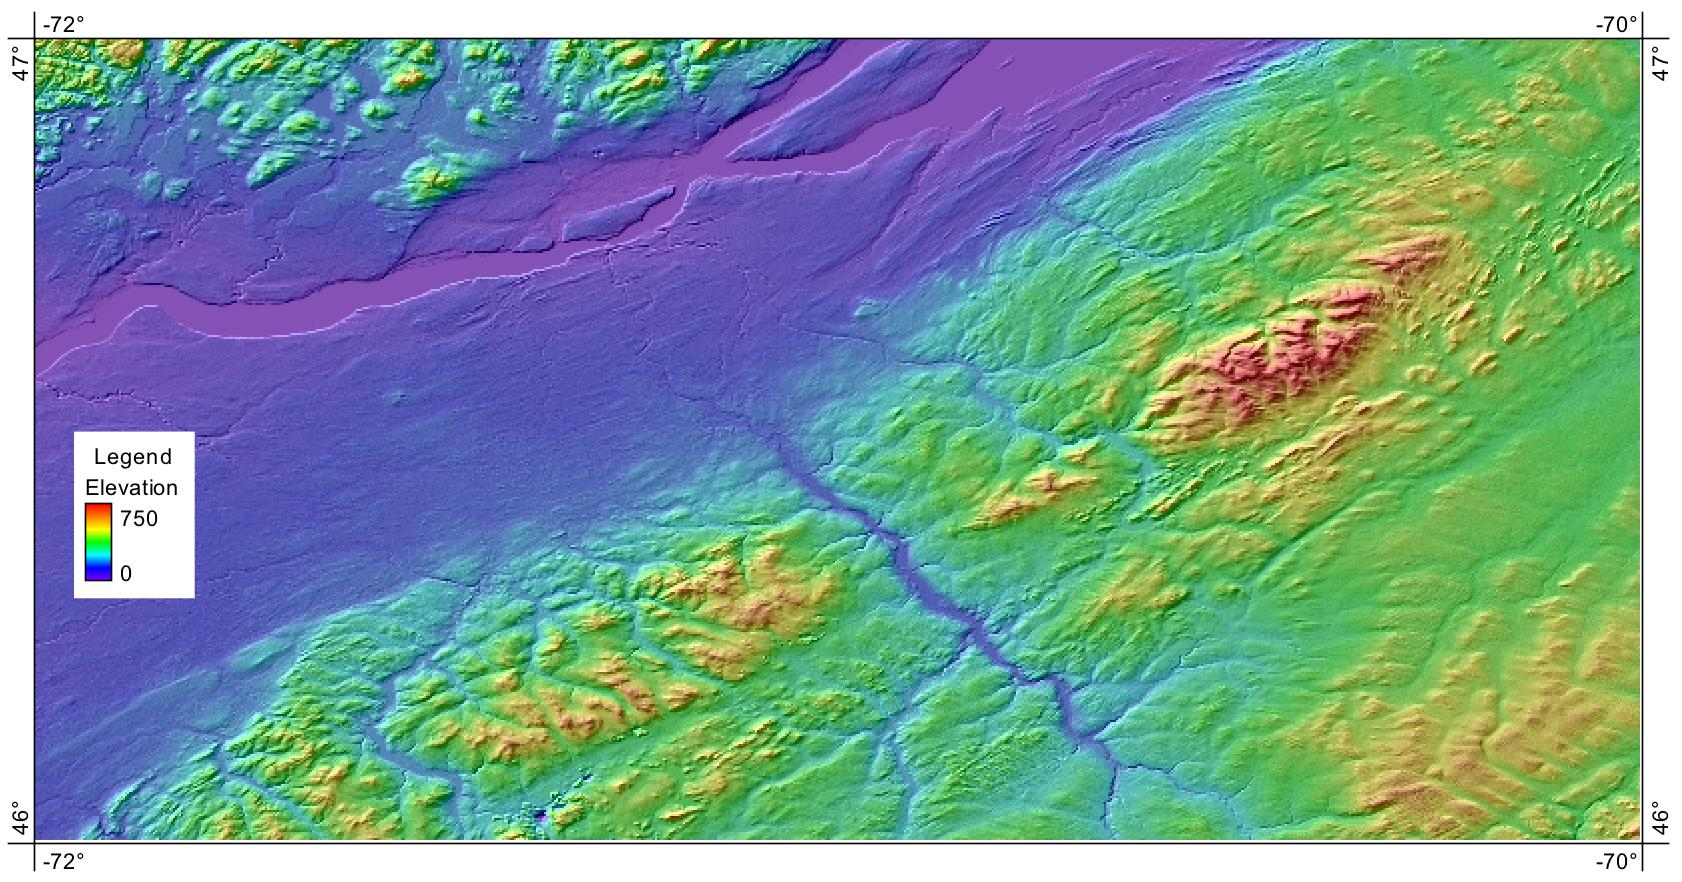
\includegraphics[height=8cm]{figures/terraincoloring.jpg}
	\caption[Coloreado de terreno por alturas.]{Coloreado de terreno por
	alturas. Fuente:~\cite{terraincoloringimage}}
	\label{fig:terrain}
\end{figure}

\section{Line Integral Convolution}
\label{ref:lic}

La última de las técnicas de visualización que vamos a ver tiene que ver con la
visualización de fluidos en dos dimensiones. Para ello veremos un método
importante denominado Line Integral Convolution.

El método Line Integral Convolution fue originalmente propuesto en el artículo
de~\citet{osti_10185520}. Se utiliza para visualizar campos vectoriales densos.
En este método, se utiliza una imagen junto con datos de un flujo vectorial,
modificando esta imagen para mostrar el flujo de los datos. (ver
Figura~\ref{fig:lic}). 

\begin{figure}[h!]
	\centering	
	\begin{subfigure}{.45\textwidth}
		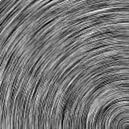
\includegraphics[height=5cm,width=\textwidth]{figures/lic2.png}
	\end{subfigure}
	\hfill
	\begin{subfigure}{.45\textwidth}
		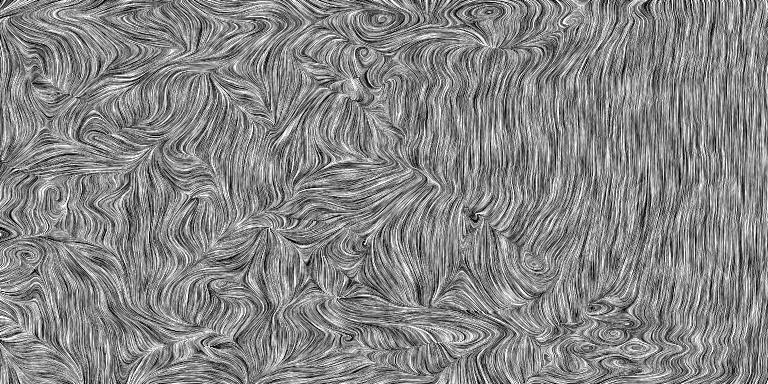
\includegraphics[height=5cm,width=\textwidth]{figures/lic1.png}
	\end{subfigure}
	\caption[Resultado del método Line Integral Convolution.]{Resultado del
			método Line Integral Convolution. Fuente:~\cite{osti_10185520}}
	\label{fig:lic}
\end{figure}

En~\citet{licthesis} se muestra como funciona el método de Line Integral
Convolution, señalando los principales pasos que sigue:

Para cada pixel en la imagen de entrada, hacer:
\begin{enumerate}
		\item Computar la línea de flujo \textit{(streamline)} para una longitud
				determinada por el usuario en direcciones positivas y
				negativas. (Figura~\ref{fig:licstreamline})
		\item \label{ref:licpaso2} Para cada punto en la streamline, computar su
				peso de convolución $h_i$. (Figura~\ref{fig:licweights})
		\item Computar el valor de salida del pixel con los valores de entrada y
				los pesos computados en~\ref{ref:licpaso2}.
				(Figura~\ref{fig:licoutputpixel})
\end{enumerate}

\begin{figure}
		\centering
		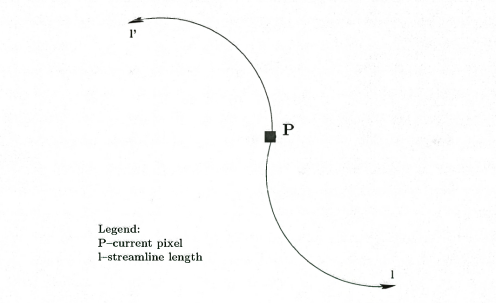
\includegraphics[height=9cm]{figures/licstreamline.png}
		\caption[Computar la línea de flujo.]{Computar la línea de flujo.
		Fuente:~\cite{licthesis}}	
		\label{fig:licstreamline}
\end{figure}

\begin{figure}
		\centering
		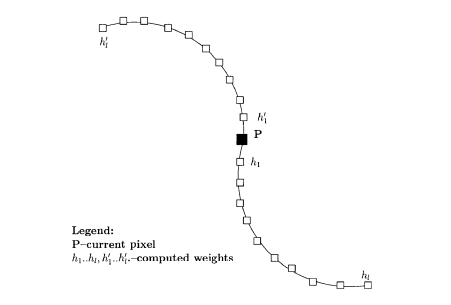
\includegraphics[height=9cm]{figures/licweights.png}
		\caption[Computar los pesos.]{Computar los pesos.
		Fuente:~\cite{licthesis}}	
		\label{fig:licweights}
\end{figure}

\begin{figure}
		\centering
		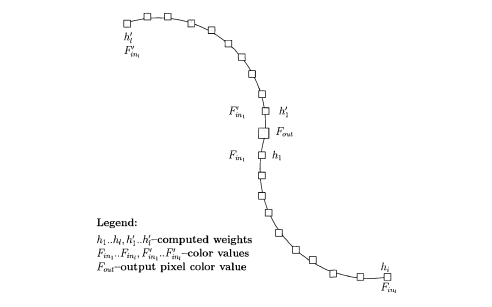
\includegraphics[height=9cm]{figures/licoutputpixel.png}
		\caption[Computar valores de salida del pixel.]{Computar valores de
		salida del pixel. Fuente:~\cite{licthesis}}	
		\label{fig:licoutputpixel}
\end{figure}

Como imagen de entrada se puede utilizar, realmente, cualquier imagen,
haciendo ver las líneas de flujo con los colores de la imagen original. Sin
embargo, con el fin de que perturbaciones en la imagen original no condicionen
el análisis del flujo a visualizar, la opción recomendada y casi siempre
utilizada en este método es la del ruido blanco, debido a la distribución
uniforme de los colores de sus píxeles. 

\subsection{Computar la línea de flujo}
\label{ref:streamline}

Para computar la línea de flujo se ha de utilizar algún método numérico. Entre
las posibilidades se encuentran el método de Euler, utilizado
por~\citet{licthesis}, el método de Euler de paso variable, utilizado por los
autores originales en~\citet{osti_10185520}, o el método de Runge-Gutta de orden
4, propuesto como alternativa en ambos textos. En la
sección~\ref{makereference5.4.3}, se explican estos métodos como preparación
para su implementación. De esta manera, se consiguen una serie de puntos a lo
largo de la línea de flujo, dependiendo del paso escogido en el método numérico
y la longitud de la línea escogida por el usuario.

\subsection{Computar los pesos de convolución}
\label{ref:convolution}

Este paso consiste en encontrar la integral exacta del núcleo de convolución $k$
en cada punto de la línea de flujo computado en el paso anterior. Es decir, se
ha de resolver la integral~\eqref{eq:11}.

\begin{equation}
		h_i = \int_{a}^{b}k(\omega) d\omega \label{eq:11}
\end{equation}

donde $i$ se representa el índice del punto actual en la línea de flujo, $a$
es la distancia a lo largo de la línea de flujo entre el punto actual y el pixel
para el que queremos calcular el valor de salida y $b$ es igual a $a$ más el
tamaño del paso utilizado en el paso actual $\Delta s_i$. Más información acerca
del núcleo de convolución puede encontrarse en~\citet{osti_10185520}.

\subsection{Computar los valores de salida del pixel}
\label{ref:salida}

Para calcular los valores de salida del pixel una vez calculados los pesos de
los puntos de la línea de flujo, se sigue la siguiente ecuación:

\begin{equation}
		F_{out}(x,y) =
		\frac{\sum\limits_{i=0}^{l}{F_{in}(P_i)h_i}+\sum\limits_{i=0}^{l'}{F_{in}(P'_i)h'_i}}{\sum\limits_{i=0}^{l}{h_i} + \sum\limits_{i=0}^{l'}{h'_i}} \label{eq:12}
\end{equation}
